% !TEX root = esm_architecture.tex

\documentclass[11pt]{article}

\usepackage[T1]{fontenc}
\usepackage{lmodern}        % cleaner font
\usepackage{microtype}      % better spacing
\usepackage{amsmath, amssymb}
\usepackage{graphicx}
\usepackage[hypertexnames=false]{hyperref}
\usepackage{geometry}
\usepackage{setspace}
\usepackage{titlesec}
\usepackage{amsthm}
\usepackage{listings}
\usepackage{xcolor}
\usepackage{float}
\usepackage{booktabs}
\usepackage{tikz}
\usetikzlibrary{arrows.meta, positioning, calc}
\usepackage{fancyhdr}
\pagestyle{fancy}
\fancyhf{}

% --- Paper versioning ---
\renewcommand{\headrulewidth}{0.4pt}
\renewcommand{\footrulewidth}{0pt}

% fallback values (used if git_version.tex is missing)
\providecommand{\paperVersion}{draft}
\providecommand{\paperDate}{\today}

\renewcommand{\paperVersion}{v1.3.0}
\renewcommand{\paperDate}{March 20, 2026}


\lhead{Richard Hines}
\rhead{ESM -- Version \paperVersion}
\cfoot{\thepage}
\rfoot{\paperDate}

\date{}


% ----------------------------
% Layout
% ----------------------------

\geometry{margin=1.15in}
\setlength{\headheight}{14pt}
\onehalfspacing

\titleformat{\section}
  {\Large\bfseries}
  {\thesection}{0.5em}{}

% ----------------------------
% Theorem environments
% ----------------------------

\newtheorem{definition}{Definition}

% ----------------------------
% Listings (Pseudocode)
% ----------------------------

\lstset{
  basicstyle=\ttfamily\small,
  frame=single,
  columns=fullflexible,
  keepspaces=true,
  showstringspaces=false,
  xleftmargin=1em,
  xrightmargin=1em,
  aboveskip=1em,
  belowskip=1em
}

% ----------------------------
% Title
% ----------------------------
\title{The Emergent State Machine:\\
An Architectural Framework for\\
Deterministic, Interpretable, Governable Decision Systems}

\author{
Richard Hines\\
\small Independent Researcher\\
\small Tacoma, Washington, USA\\
\small \texttt{richardhinestacoma@gmail.com}\\
}

\begin{document}

\maketitle

\begin{abstract}

The Emergent State Machine (ESM) is a deterministic architectural framework for interpretable situational reasoning in complex domains. The architecture structures reasoning as a sequence of explicit, inspectable steps in which situational meaning is constructed as explicit state prior to any consideration of action.

Within each turn, raw observations are transformed into signals, which are assembled into a coherent, committed state representation of the current situation. This state is then expressed in policy-relevant coordinates through projection, evaluated for relevance via explicit gating, and, when warranted, acted upon through deterministic policy. This sequence enforces a structural separation between state construction (interpretation), projection, relevance gating, and authoritative policy action. Traceability is formalized as a causal chain 
$r_t \leftarrow g_t \leftarrow y_t \leftarrow x_t \leftarrow S_t \leftarrow o_t$,
making each decision reconstructable from its underlying observations, signals, and policy logic.

ESM provides a structured deployment and calibration pathway that enables safe onboarding into existing environments. Initial ``lights-on'' observation-only mode ($g_t=0$) validates representations without operational risk, followed by multi-projection preference elicitation and progressive policy activation (Section~\ref{sec:deployment}).

By organizing behavior as a sequence of turns, the ESM makes state evolution visible as trajectories through interpretable and policy-relevant state spaces, so that longer-run behavior can be analyzed in terms of policy-defined desirable and undesirable regions, without implying global trajectory optimization. 

The architecture establishes a deterministic boundary at the point of decision, ensuring that all outcomes arise only after a fully constructed situational state, and that actions occur exclusively through authorized policy evaluation. Because signals, projections, gating logic, and policies are explicitly defined and versioned, system behavior can evolve only through intentional, versioned modification of these architectural artifacts. The reasoning that produces each decision is explicitly structured, inspectable, and accountable, rather than an opaque internal process. This approach addresses a central limitation of contemporary decision systems, in which responsibility for consequential decisions remains with human operators while the computational processes supporting those decisions often remain uninspectable. 

The canonical specification of the architecture is available at the
\href{https://github.com/emergent-state-machine/esm-spec}{ESM specification repository on GitHub}\footnote{\url{https://github.com/emergent-state-machine/esm-spec}}.

\subsection*{Contributions}

This paper introduces the Emergent State Machine (ESM), a deterministic architectural framework for structuring interpretable situational reasoning. The architecture formalizes reasoning as a sequence of turns in which observations are transformed into signals and assembled into a coherent, committed state representation prior to any evaluation of action. Decisions arise only after this state is fully constructed; when relevance gating permits, policy is invoked to produce the turn outcome, and otherwise the turn resolves as an explicit no-op.

A central contribution of the architecture is the explicit separation between state construction (interpretation), projection, relevance gating, and policy action. This separation constrains where and how state mutation can occur, ensuring that interpretation is completed before decision evaluation and that policy is the sole mechanism by which action is authorized. As a result, system behavior is traceable to explicit architectural components rather than embedded within opaque transformations.

The framework provides a \emph{structured deployment pathway} supporting safe onboarding into existing environments: observation-only validation ($g_t=0$), multi-projection calibration via expert preference elicitation, and progressive policy activation from shadow mode to full authority (Section~\ref{sec:deployment}).

The framework further formalizes system behavior as trajectories through interpretable and policy-relevant state spaces over discrete turns. Policy-defined regions of desirability provide a way to describe longer-run behavior in terms of where trajectories tend to remain or return, without positing global optimization.

Because signals, projections, relevance determination logic, and policies are explicitly defined and versioned, the architecture supports Instrumented Deterministic Evolution, in which behavioral change occurs only through intentional modification of versioned system components. This enables systematic testing, comparison, and refinement of system behavior over time.

Finally, the architecture supports composition across temporal scales via layered ESMs and explicit state handoff, allowing multiple interacting systems to maintain local reasoning, shared context, and deterministic authority without loss of modularity or provenance.

\end{abstract}

% ----------------------------
% Introduction
% ----------------------------
\section{Introduction}

Contemporary decision systems often operate as opaque pipelines where complex transformations produce outputs without exposing reasoning steps. In domains like clinical care, education, and operational control, professionals bear responsibility for consequential decisions while computational support remains uninspectable. Threshold alerting surfaces measurements but leaves operators to reconstruct situational context themselves \cite{endsley1995}.

The Emergent State Machine (ESM) structures reasoning as discrete \emph{turns}, each committing to a coherent state $x_t$ before any action consideration. 


\begin{center}
\small
\[
\begin{aligned}
\textbf{Observations} &\;\longrightarrow\; \textbf{Signals} \;\longrightarrow\; \textbf{Coherent State Vector} \;\longrightarrow\; \textbf{Projection} \\
&\qquad\;\longrightarrow\; \textbf{Relevance} \;\longrightarrow\; \textbf{Policy} \;\longrightarrow\; \textbf{Outcome}
\end{aligned}
\]
\end{center}

\vspace{-0.5em}
\begin{center}
\small Figure~\refstepcounter{figure}\thefigure: Canonical ESM pipeline.
\label{fig:esm-canonical-pipeline}
\end{center}


Each turn formalizes the causal chain
\[
r_t \leftarrow g_t \leftarrow y_t \leftarrow x_t \leftarrow S_t \leftarrow o_t.
\]
State construction completes interpretation as a fully resolved situational construct. Projection re-expresses this state in policy coordinates without semantic alteration. Gating determines whether policy evaluation is invoked; policy alone produces actions. Interpretation precedes gating precedes action.

System evolution manifests as trajectories $\{x_1, x_2, \dots\}$ through policy-relevant state space, arising from locally governed turns rather than global optimization. Time advances discretely via completed commitments, with turns occurring at decision-relevant moments rather than uniform observation intervals.

Key properties:
\begin{itemize}
\item \textbf{Committed turns}: Complete reasoning frames, inspectable in isolation or sequence
\item \textbf{Deterministic boundary}: Policy is sole action authority, activated only by gating
\item \textbf{Explicit artifacts}: Signals, projections, gating, policies are versioned and auditable
\item \textbf{Instrumented evolution}: Behavioral change occurs only through governed revision (Section~\ref{sec:IDE})
\item \textbf{Structured deployment}: Safe onboarding via phased calibration and activation (Section~\ref{sec:deployment})
\item \textbf{Layered composition}: ESMs interoperate via explicit state handoff (Section~\ref{sec:layered_esms})
\end{itemize}

This yields computational reasoning where every outcome traces to specific state, authorization boundary, and policy evaluation. The canonical specification---defining deterministic execution such that identical inputs yield identical outcomes---is at \href{https://github.com/emergent-state-machine/esm-spec}{github.com/emergent-state-machine/esm-spec}. A reference implementation is under active development.

% ----------------------------
% ESM as a Discrete-Time System
% ----------------------------

\section{ESM as a Discrete-Time System}

The ESM operates as a discrete-time system where time advances through completed turns. Each turn $T_t$ constitutes a full reasoning frame, committing to state $x_t$ before any action consideration.

At turn $t$, observations $o_t$ produce signals $S_t \to$ committed state $x_t \to$ projection $y_t \to$ gating $g_t \to$ policy outcome $r_t$, formalized as the causal chain:
\[
r_t \leftarrow g_t \leftarrow y_t \leftarrow x_t \leftarrow S_t \leftarrow o_t.
\]

Unlike continuous dynamical systems with implicit state evolution, ESM advances through explicit commitments at discrete decision boundaries. Time indexes completed reasoning steps, not continuous flow.

Outcomes $r_t$ (including explicit no-op) shape turn $t+1$ via environmental effects or state handoff in layered ESMs. Trajectories $\{x_1, x_2, \dots\}$ emerge from locally governed decisions, not global optimization.

Policy remains the sole mechanism producing actions, ensuring that interventions follow explicit architectural constraints rather than hidden dynamics. Each turn's inspectability enables trajectory analysis without assuming optimal control.


% ----------------------------
% The Turn as the Fundamental Unit of Computation
% ----------------------------

\section{The Turn as the Fundamental Unit of Computation}

The turn $T_t = (o_t, S_t, x_t, y_t, g_t, r_t)$ is the atomic reasoning object: a complete, inspectable frame committing to state $x_t$ before policy consideration.

State mutation occurs only at turn conclusion via the outcome $r_t$, which is determined by gating and, when invoked, policy. Each turn constrains subsequent evolution through its committed state and outcome.

\begin{itemize}
\item $o_t$: observations at time $t$
\item $S_t$: signals computed from $o_t$
\item $x_t$: committed state vector
\item $y_t$: projection ($P(x_t)$) into policy coordinates (no semantic alteration)
\item $g_t$: gating signal authorizing policy evaluation
\item $r_t$: authorized outcome (no-op, action, escalation, handoff, clarification)
\end{itemize}

Policy produces outcomes only when invoked ($g_t = 1$), and is the sole mechanism producing actions. Every turn constitutes a complete, auditable decision record exposing the full causal chain.

Initialization establishes $x_0$ from structured inputs (intake, prior outputs, baselines), ensuring the first turn begins from explicit context rather than empty state.

Sequences $\{T_1, T_2, \dots\}$ form reconstructible trajectories for analysis. The turn structure is domain-invariant: clinical ESMs use physiological signals/treatment policies; manufacturing uses process signals/control policies. The computational scaffold remains identical.

Generalization arises from reusing this fixed turn structure across domains via redefined, versioned signals/projections/policies, not parameter adaptation within models.

\vspace{0.5em}
\begin{figure}[H]
\centering
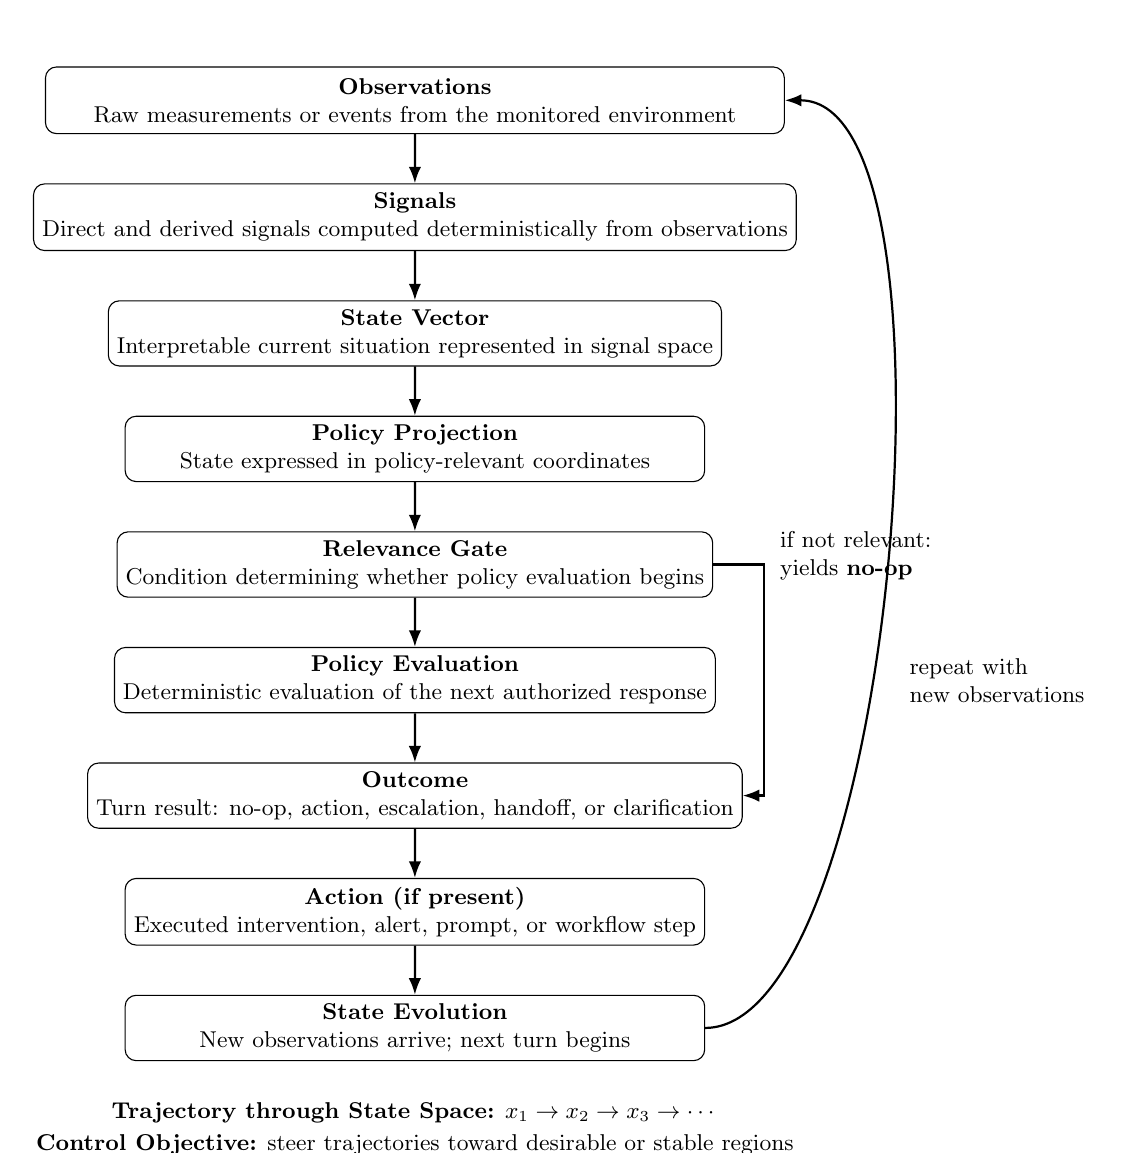
\begin{tikzpicture}[
  scale=0.92,
  transform shape,
  node distance=0.68cm,
  box/.style={
    rectangle,
    rounded corners,
    draw,
    align=center,
    minimum width=10.2cm,
    minimum height=0.92cm,
    font=\small
  },
  smallbox/.style={
    rectangle,
    rounded corners,
    draw,
    align=center,
    minimum width=8.0cm,
    minimum height=0.84cm,
    font=\small
  },
  note/.style={
    align=left,
    font=\small
  },
  arrow/.style={
    -{Latex[length=2.1mm]},
    thick
  }
]

% Main vertical chain
\node[box] (obs) {\textbf{Observations}\\Raw measurements or events from the monitored environment};

\node[box, below=of obs] (sig) {\textbf{Signals}\\Direct and derived signals computed deterministically from observations};

\node[smallbox, below=of sig] (state) {\textbf{State Vector}\\Interpretable current situation represented in signal space};

\node[smallbox, below=of state] (proj) {\textbf{Policy Projection}\\State expressed in policy-relevant coordinates};

\node[smallbox, below=of proj] (gate) {\textbf{Relevance Gate}\\Condition determining whether policy evaluation begins};

\node[smallbox, below=of gate] (policy) {\textbf{Policy Evaluation}\\Deterministic evaluation of the next authorized response};

\node[smallbox, below=of policy] (outcome) {\textbf{Outcome}\\Turn result: no-op, action, escalation, handoff, or clarification};

\node[smallbox, below=of outcome] (action) {\textbf{Action (if present)}\\Executed intervention, alert, prompt, or workflow step};

\node[smallbox, below=of action] (evolve) {\textbf{State Evolution}\\New observations arrive; next turn begins};

% Main arrows
\draw[arrow] (obs) -- (sig);
\draw[arrow] (sig) -- (state);
\draw[arrow] (state) -- (proj);
\draw[arrow] (proj) -- (gate);
\draw[arrow] (gate) -- (policy);
\draw[arrow] (policy) -- (outcome);
\draw[arrow] (outcome) -- (action);
\draw[arrow] (action) -- (evolve);

% Gate side note for no-op
\node[note, right=0.8cm of gate, yshift=0.12cm] (gatenote) {if not relevant:\\yields \textbf{no-op}};
\draw[arrow] (gate.east) -- ++(0.7,0) |- (outcome.east);

% Loop back
\draw[arrow] (evolve.east) .. controls +(2.6,0) and +(2.6,0) .. (obs.east);

% Loop label
\node[note, right=2.55cm of policy] {repeat with\\new observations};

% Bottom summary text
\node[align=center, below=0.45cm of evolve, font=\small] (traj)
{\textbf{Trajectory through State Space:} $x_1 \rightarrow x_2 \rightarrow x_3 \rightarrow \cdots$\\[0.15em]
\textbf{Control Objective:} steer trajectories toward desirable or stable regions};

\end{tikzpicture}

\caption{Turn structure: $o_t \to S_t \to x_t \to y_t \to g_t \to r_t$. An outcome is produced on every turn (including explicit no-op); actions occur only when $g_t = 1$.}
\label{fig:esm-core-loop}
\end{figure}

% ----------------------------
% From Observations to Signals
% ----------------------------
\section{From Observations to Signals}

Signals $S_t$ define the system's representational capacity: explicit, deterministic distinctions over observations $o_t$ that determine what can be known, tracked, and acted upon.

\subsection{Direct Signals}
Direct signals extract values from $o_t$:
\begin{equation}
s_i^{\mathrm{direct}} = m_i(o_t)
\end{equation}
where $m_i$ is a deterministic measurement function (e.g., heart rate, respiratory rate, student response).

\subsection{Derived Signals}
Derived signals compute relationships over observations or prior signals:
\begin{equation}
s_j^{\mathrm{derived}} = f_j(o_t, o_{t-k:\,t-1}, S_{t-1})
\end{equation}
where $f_j$ formalizes domain knowledge (ratios, trends, persistence, shock index $\frac{HR}{SBP}$).

\subsection{Signal Set}
The complete set is $S_t = S_t^{\mathrm{direct}} \cup S_t^{\mathrm{derived}}$, grounding all subsequent state construction and policy evaluation.

Signals are designed distinctions, not neutral measurements. Their definitions determine representational capacity---what's visible to reasoning is exactly what's captured as signals. Undetected patterns remain invisible by architectural constraint.

Signal design is governance: choices shape detection, relationships, and actionability. Signals are deterministic, versioned, and auditable, enabling controlled evolution via Instrumented Deterministic Evolution (IDE).

$S_t$ forms the explicit interface between raw $o_t$ and committed state $x_t$, operationalizing domain knowledge as executable structure.

% ----------------------------
% Constructing the Committed State
% ----------------------------

\section{Constructing the Committed State}

The state $x_t$ is a coherent, committed representation of the current situation, constructed from signals $S_t$ via explicit organizational rules for decision relevance.

Formally,
\begin{equation}
x_t = (s_1, s_2, \dots, s_n), \quad s_i \in S_t
\end{equation}
where components are heterogeneous (numeric, categorical, uncertainty indicators) with explicitly known definitions, types, and scales---no vector space operations assumed.

The state vector is constructed anew on each turn from current observations together with the consequences of prior turns. It represents a fresh, fully coherent situational commitment rather than an incremental mutation of a previously stored state.

All components describe the same moment, interpreted together as a fully resolved situational construct. Interpretation completes here; no partial estimates or latent inference. Downstream components operate on this committed representation.

Deterministic construction from versioned signals ensures identical inputs produce identical $x_t$, enabling audit and replay.

% ----------------------------
% Relevance Determination
% ----------------------------
\section{Relevance Determination via Gating}

Gating $g_t = G(y_t) \in \{0,1\}$ determines whether policy evaluation is invoked for projected state $y_t$. The system always constructs state, but policy is evaluated only when $g_t = 1$.

If $g_t = 1$, policy $\pi(y_t)$ is evaluated and produces outcome $r_t$. If $g_t = 0$, policy is not invoked and the outcome $r_t$ is an explicit no-op. Every turn evaluates; not every turn acts.

\begin{figure}[H]
\centering
\centering
\resizebox{\linewidth}{!}{
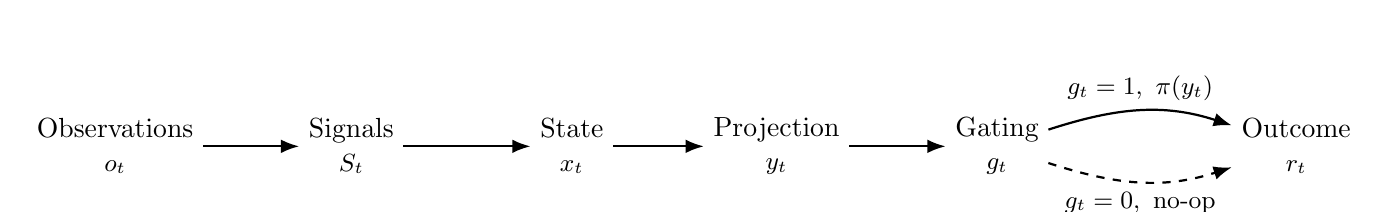
\begin{tikzpicture}[
    >=Latex,
    lbl/.style={font=\normalsize, align=center},
    ann/.style={font=\small},
    flow/.style={->, thick},
    noflow/.style={->, dashed, thick}
]

% Main pipeline labels
\node[lbl] (o) at (0,0) {Observations \\ {\small $o_t$}};
\node[lbl] (S) at (3.0,0) {Signals \\ {\small $S_t$}};
\node[lbl] (x) at (5.8,0) {State \\ {\small $x_t$}};
\node[lbl] (y) at (8.4,0) {Projection \\ {\small $y_t$}};
\node[lbl] (g) at (11.2,0) {Gating \\ {\small $g_t$}};
\node[lbl] (r) at (15.0,0) {Outcome \\ {\small $r_t$}};

% Main left-to-right pipeline
\draw[flow] (o) -- (S);
\draw[flow] (S) -- (x);
\draw[flow] (x) -- (y);
\draw[flow] (y) -- (g);

% g_t = 1 branch (solid)
\draw[flow] (g) to[out=18,in=162] node[midway, above, ann] {$g_t = 1,\ \pi(y_t)$} (r);

% g_t = 0 branch (dashed)
\draw[noflow] (g) to[out=-18,in=-162] node[midway, below, ann] {$g_t = 0,\ \text{no-op}$} (r);

\end{tikzpicture}
}

\caption{Relevance determination by gating. Observations are transformed into signals, composed into a state, and projected into policy-relevant coordinates before reaching gating $g_t$. From this decision boundary, the turn branches to a shared outcome $r_t$: when $g_t=1$, policy $\pi(y_t)$ is invoked; when $g_t=0$, the turn yields an explicit no-op outcome without policy invocation.}
\label{fig:esm-gating-pipeline}
\end{figure}

Gating operates solely on $y_t$, ensuring consistent decision coordinates. Conditions may include thresholds, persistence, region transitions, volatility, or composite relationships---not limited to single-signal exceedance.

Gating separates continuous state construction from conditional intervention. Explicit $G$ functions are inspectable: any turn's activation can be traced to specific $y_t$ conditions.

Multi-policy configurations use multiple $G_i(y_t)$, preserving deterministic invocation independent of policy logic. Gating establishes invocation determinism: both when decisions occur and their outcomes are governed explicitly.

\section*{8 \quad Policy and Authorized Outcomes}
\label{sec:policy}

Policy $\pi(y_t)$ is the sole mechanism producing non-trivial outcomes $r_t$, and is invoked only when gating permits ($g_t = 1$).

\begin{align}
g_t &= 0 \quad \Rightarrow \quad r_t = \mathrm{no\text{-}op} \\
g_t &= 1 \quad \Rightarrow \quad r_t = \pi(y_t) \quad (a_t \in \{\text{action, escalation, handoff, clarification}\})
\end{align}

No-op is explicit: when $g_t = 0$, policy is not invoked and the outcome is deterministically no-op. When $g_t = 1$, policy $\pi(y_t)$ is invoked and may produce either action or no-op depending on defined rules.

Complete causal chain:
\begin{equation}
r_t \leftarrow g_t \leftarrow y_t \leftarrow x_t \leftarrow S_t \leftarrow o_t
\end{equation}

Deterministic $\pi$ ensures identical $y_t$ yields identical $r_t$. All prior stages establish situation and relevance; only policy authorizes action.

% ----------------------------
% Projection into Policy Space
% ----------------------------

\section{Projection into Policy Space}
\label{sec:projection}

Projection $y_t = P(x_t)$ re-expresses the committed state $x_t$ in policy-relevant coordinates without introducing new semantic content. Interpretation completes at state construction; projection enables decision evaluation.

$P$ is a deterministic transformation (linear, nonlinear, or model-assisted) whose definition remains explicit and inspectable. Policy operates solely on $y_t$, never directly on raw signals or unprojected state.

Each component of $y_t$ represents a policy-relevant dimension (e.g., respiratory instability, claim strength, confidence, volatility) defined by domain experts. Confidence or uncertainty may be included as explicit coordinates, computed deterministically or via reproducible models.

Projection separates situational description from decision framing:
\begin{itemize}
    \item $x_t$: what is happening (coherent situational construct)
    \item $y_t$: how it matters for policy (decision coordinates)
\end{itemize}

Changes to $P$ revise decision coordinates explicitly via versioned artifacts, preserving inspectability. Gating $G(y_t)$ and policy $\pi(y_t)$ operate in a consistent coordinate system.

\begin{figure}[H]
\centering
% Figure: worked example of coherent state and projection
% Requires in preamble:
% \usepackage{tikz}
% \usetikzlibrary{positioning,arrows.meta}

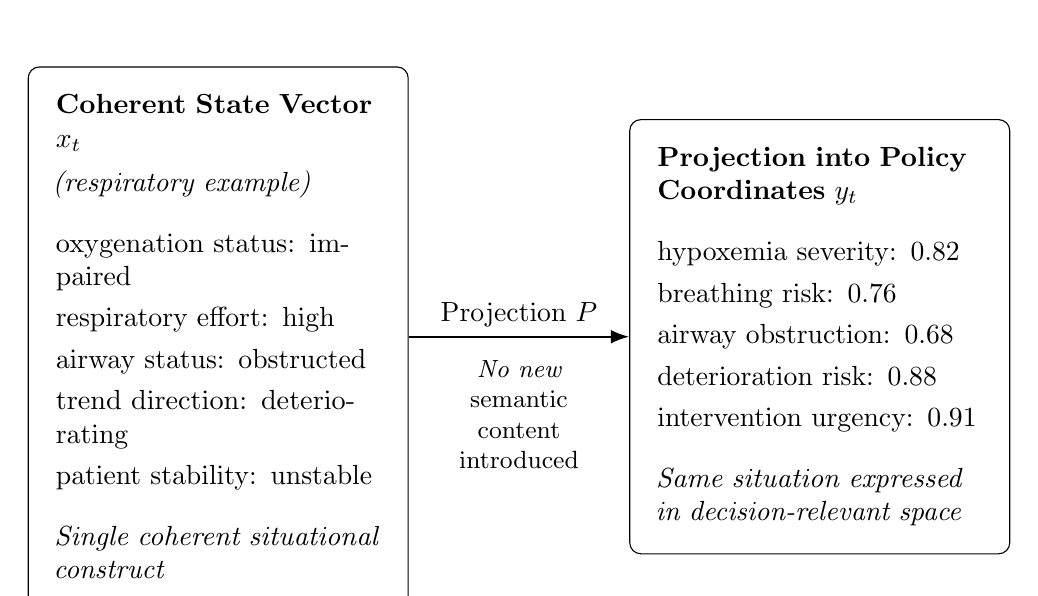
\begin{tikzpicture}[
    >=Latex,
    box/.style={
        draw,
        rounded corners=4pt,
        align=left,
        text width=0.34\textwidth,
        inner sep=10pt,
        minimum height=4.8cm
    },
    note/.style={align=center, font=\small}
]

\node[box] (state) {
{\bfseries Coherent State Vector $x_t$}\\[4pt]
{\itshape (respiratory example)}\\[10pt]
oxygenation status: impaired\\[3pt]
respiratory effort: high\\[3pt]
airway status: obstructed\\[3pt]
trend direction: deteriorating\\[3pt]
patient stability: unstable\\[10pt]
{\itshape Single coherent situational construct}
};

\node[box, right=2.8cm of state] (proj) {
{\bfseries Projection into Policy Coordinates $y_t$}\\[10pt]
hypoxemia severity: 0.82\\[3pt]
breathing risk: 0.76\\[3pt]
airway obstruction: 0.68\\[3pt]
deterioration risk: 0.88\\[3pt]
intervention urgency: 0.91\\[10pt]
{\itshape Same situation expressed in decision-relevant space}
};

\draw[->, thick] (state.east) -- node[above, font=\normalsize] {Projection $P$} (proj.west);

\node[note, below=5pt of $(state.east)!0.5!(proj.west)$] {\itshape No new \\semantic \\content \\introduced};

\end{tikzpicture}

\caption{Worked example of state construction and projection in a respiratory ESM. The coherent state vector $x_t$ represents a fully resolved situational construct. Projection maps that same situation into policy-relevant coordinates $y_t$ without introducing new semantic content, enabling downstream relevance evaluation and policy to operate on an explicitly defined decision space.}
\label{fig:state-projection-example}
\end{figure}

\subsection{Lights-On Projection Validation}

ESM supports a \emph{lights-on} validation mode in which projection is evaluated prior to policy activation. In this mode, gating is disabled ($g_t = 0$), ensuring that no actions are authorized while projection behavior is inspected.

This separation allows domain experts to assess whether projected coordinates $y_t$ appropriately reflect decision-relevant structure without introducing operational risk. Projection outputs can be examined, compared, and iteratively refined before enabling policy execution.

Formally, projection remains unchanged:
\begin{equation}
y_t = P(x_t)
\end{equation}

but system operation is constrained to observation-only evaluation:
\begin{equation}
g_t = 0 \quad \Rightarrow \quad r_t = \mathrm{no\text{-}op}
\end{equation}

This establishes a clear boundary between \emph{representation validation} (projection) and \emph{decision authorization} (policy), enabling controlled system introduction in real-world environments.

% ----------------------------
% Deployment and Calibration
% ----------------------------
\section{Deployment and Calibration}
\label{sec:deployment}

ESM is typically layered into existing environments where decision practices and partial workflows are already established. Deployment therefore emphasizes \emph{alignment and calibration} rather than from-scratch specification.

ESM provides a structured onboarding pathway that separates representation validation, preference elicitation, and policy activation into distinct phases.

\subsection{Observation-Only Initialization (Lights-On Mode)}

Deployment begins in \emph{lights-on} (observation-only) mode with action authority withheld ($g_t = 0$):

\begin{equation}
g_t = 0 \quad \Rightarrow \quad r_t = \mathrm{no\text{-}op}
\end{equation}

The representation pipeline processes real inputs, making $x_t$ and $y_t$ visible to practitioners without operational risk. This phase establishes trust in signal processing, state construction, and projection before any intervention authority is granted.

\subsection{Projection Calibration}

Multiple candidate projection views ${P_i}$---each encoding different organizational priorities---are applied to the same committed state $x_t$:

\begin{equation}
y_t^{(i)} = P_i(x_t), \quad i \in {1, \dots, k}
\end{equation}

where $P_i$ represents distinct projection policies (safety-oriented, throughput-oriented, cost-aware, equity-aware, etc.).

These alternatives appear side-by-side, allowing domain experts to compare interpretations of identical situations rather than specifying abstract rules from scratch.

\subsection{Preference Elicitation}

Experts indicate preferences over projection variants via simple interfaces (tap, swipe, thumbs-up/down). This approach sidesteps the cognitive difficulty of articulating complete decision logic by focusing on relative merit.

Preference patterns provide structured data for:
\begin{itemize}
\item Implicit extraction of organizational decision priorities
\item Identification of signal or projection gaps
\item Iterative refinement of projection functions $P_i(\cdot)$
\end{itemize}

Selected projections narrow the space of plausible downstream policies while operating on decision-relevant representations rather than raw signals.

\subsection{Progressive Policy Activation}

With validated representations and aligned projections, the system advances through staged activation:

\begin{itemize}
\item \textbf{Shadow mode}: Policy $\pi(y_t)$ computes outputs that are logged but not executed
\item \textbf{Advisory mode}: Recommendations appear without enforcement authority
\item \textbf{Partial activation}: Policy applies to specific cases, domains, or risk thresholds
\item \textbf{Full activation}: $g_t = 1$ authorizes committed outcomes $r_t$
\end{itemize}

\subsection{Integration with Existing Systems}

ESM formalizes decision structure without replacing upstream data sources or downstream execution systems. Signals $S_t$ may derive from legacy feeds; policy outcomes $r_t$ may integrate with existing escalation, review, or actuation mechanisms.

This compatibility supports incremental adoption while delivering deterministic structure, auditability, and explicit decision boundaries.

\subsection{Summary}

ESM deployment follows a controlled progression: observe representations, calibrate projections via expert preference, then gradually activate policy authority. This pathway reduces specification burden, preserves interpretability, and enables layering into complex operational environments.

% ----------------------------
% State Evolution and Trajectories
% ----------------------------
\section{State Evolution and Trajectories}

State evolution proceeds through successive turns: $x_{t+1} = \Phi(x_t, o_{t+1})$, where $\Phi$ deterministically constructs committed state from new observations and explicit context (derived signals, initialization).

Trajectories form as observable sequences:
\begin{align}
\{x_1, x_2, \dots\}, \quad \{y_1, y_2, \dots\}, \quad \{T_1, T_2, \dots\}
\end{align}

Real-world time between turns varies; temporal structure enters via derived signals (trends, persistence, decay). No continuous dynamics---evolution occurs at discrete decision boundaries.

Trajectories arise from locally governed turns, not global optimization. Policy-defined desirable regions characterize observed patterns (convergence, persistence, divergence) without assuming attractors or optimal control.

Local evaluation constrains evolution to reachable configurations from current committed state, reflecting path dependence without dynamical systems formalism.

% ----------------------------
% Layered ESMs
% ----------------------------
\section{Layered ESMs and State Handoff}
\label{sec:layered_esms}

ESMs compose hierarchically: upstream ESMs produce initialized state $x^{(u)}_{\text{handoff}}$ for downstream ESMs.

Downstream initialization:
\begin{equation}
x^{(d)}_{1} = H\!\left(x^{(u)}_{\text{handoff}},\, o^{(d)}_{1}\right)
\end{equation}

$H$ explicitly transforms upstream state into downstream signals via deterministic rules, preserving auditability. No hidden coupling---state transfers explicitly at turn boundaries.

Key properties:
\begin{itemize}
\item \textbf{Explicit initialization}: Every ESM begins from defined $x_0$, internal or upstream
\item \textbf{Discrete handoff}: Coordination via turn outcomes and state transfer, not continuous sharing
\item \textbf{Temporal independence}: ESMs operate at different frequencies, synchronized via explicit handoffs
\item \textbf{Modularity preserved}: Local reasoning + shared context without collapsing authority
\end{itemize}

Layered ESMs enable specialized reasoning over shared context while maintaining full traceability across abstraction levels and timescales.

% ----------------------------
% Policy-Defined Desirable Regions
% ----------------------------\section{Desirable Regions and Stable States}

\section{Policy-Defined Desirable Regions}
\label{sec:desirable_regions}

Domain experts define desirable regions $\mathcal{Y}_D \subset \mathcal{Y}$ within projected state space $\mathcal{Y}$, representing preferred conditions in policy coordinates.

$\mathcal{Y}_D$ informs gating/policy design (thresholds, escalation criteria) at design time, not runtime membership checks. Projection $P$ couples to $\mathcal{Y}_D$: changes to $P$ require corresponding region revision.

Trajectories $\{y_1, y_2, \dots\}$ through policy space move toward/away from/persist near $\mathcal{Y}_D$ via world dynamics + policy outcomes. Stability is temporal: sustained residence over turns, not instantaneous points.

Examples:
\begin{itemize}
\item Clinical: sustained respiratory stability + low volatility
\item Educational: reasoning coherence + evidence alignment over turns
\end{itemize}

\begin{figure}[t]
\centering
\input{../../figures/esm-trajectories.tex}
\caption{Illustrative trajectory patterns through policy-relevant state space, showing movement relative to desirable and undesirable regions.}
\label{fig:esm-trajectories}
\end{figure}

Instrumented Deterministic Evolution (IDE) evaluates signal/projection/gating/policy revisions by trajectory behavior relative to $\mathcal{Y}_D$, enabling systematic refinement without global optimization.


% ----------------------------
% Determinism and Auditability
% ----------------------------

\section{Determinism and Auditability}
\label{sec:determinism}

Fixed versioned definitions ensure determinism: identical $o_t$ produces identical $r_t$ via the chain
\[
o_t \rightarrow S_t \rightarrow x_t \rightarrow y_t \rightarrow g_t \rightarrow r_t.
\]

\subsection{Probabilistic Components}
Model-assisted signal extraction/projection outputs become fixed explicit inputs post-capture. Stochasticity is isolated; downstream transformations remain deterministic.

\subsection{Replayability}
Recorded traces + versioned definitions reproduce complete reasoning trajectories, enabling retrospective analysis of alternative configurations.

\subsection{Failure Localization}
Undesirable $r_t$ traces to specific stage (signals, state, projection, gating, policy). Layered ESMs localize across handoff boundaries.

\subsection{Audit Record}
Every turn retains:
\begin{itemize}
\item $o_t$, $S_t$, $x_t$, $y_t$, $g_t$, $r_t$
\item versioned definitions of all transformations
\end{itemize}

Audit reconstructs \emph{how} and \emph{under which configuration} decisions occurred, enabling systematic refinement via Instrumented Deterministic Evolution.



% ----------------------------
% Governance Boundaries
% ----------------------------

\section{Governance Boundaries}

ESM produces explicit turn records $(o_t, S_t, x_t, y_t, g_t, r_t)$ for direct chain inspection, shifting interpretability from post-hoc explanation to intrinsic property.

\subsection{Human Role}
Humans define domain semantics:
\begin{itemize}
\item signals capturing measurable distinctions
\item projections framing decision coordinates  
\item desirable regions $\mathcal{Y}_D$ (Sec.~\ref{sec:desirable_regions})
\item gating thresholds and policy rules $\pi$
\end{itemize}

Teams refine independently:
\begin{itemize}
\item clinical: respiratory signals $\to$ escalation criteria $\to$ intervention policy
\item educational: reasoning signals $\to$ assessment projections $\to$ feedback rules
\end{itemize}

\subsection{AI Role}
AI assists interpretation only:
\begin{itemize}
\item signal extraction from unstructured data
\item derived signal generation  
\item projection support
\end{itemize}

AI outputs become fixed explicit inputs. No authority to commit state or authorize action.

\subsection{Authority Boundary}
Policy $\pi(y_t)$ is the sole mechanism producing actions when $g_t = 1$. Humans/AI enrich interpretation; policy governs commitment. Failure traces to a specific stage in the causal chain (Sec.~\ref{sec:determinism}).

Versioned artifacts enable targeted revision and human-system co-evolution via Instrumented Deterministic Evolution.

% ----------------------------
% Governance through Explicit Artifacts 
% ----------------------------

\section{Governance through Explicit Artifacts}

Governance in ESM targets versioned components: signals, state construction, projection $P$, gating $G$, policy $\pi$, desirable regions $\mathcal{Y}_D$. These explicit artifacts shape both representation (what's seen) and authority (what's authorized).

Governance spans all layers:
\begin{itemize}
\item \textbf{Signals}: what distinctions matter (measurement power)
\item \textbf{Projection}: decision coordinates ($x_t \to y_t$) 
\item \textbf{Gating}: when policy activates ($G(y_t)$)
\item \textbf{Policy}: what outcomes $r_t$ are authorized
\item \textbf{Desirable regions}: stability targets $\mathcal{Y}_D$
\end{itemize}

AI/human contributions (signal extraction, projection support) enter as fixed inputs. Policy $\pi(y_t)$ is the sole mechanism producing actions when $g_t = 1$. No implicit updates bypass the deterministic boundary.

Stakeholders revise independently:
\begin{itemize}
\item refine respiratory signals without changing escalation policy
\item adjust $\mathcal{Y}_D$ without modifying gating thresholds  
\item constrain policy actions without redefining projection
\end{itemize}

\section{Instrumented Deterministic Evolution (IDE)}
\label{sec:IDE}

IDE governs evolution: behavioral change occurs \emph{only} through versioned artifact revision.

\subsection{Replay Evaluation}
Recorded traces replay under config $v$:
\[
r_t^{(v)} = R^{(v)}(o_t) \quad \text{vs.} \quad r_t^{(v')} = R^{(v')}(o_t)
\]
Compare trajectories $\{T_1^{(v)}, \dots\}$ vs $\{T_1^{(v')}, \dots\}$ to assess signal/projection/gating/policy changes.

\subsection{Training Loop}
\begin{enumerate}
\item Record interaction traces
\item Train improved signal extractors/projections offline
\item Replay traces under candidate $v'$
\item Deploy $v'$ as versioned artifacts if validated
\end{enumerate}

\begin{figure}[H]
\centering
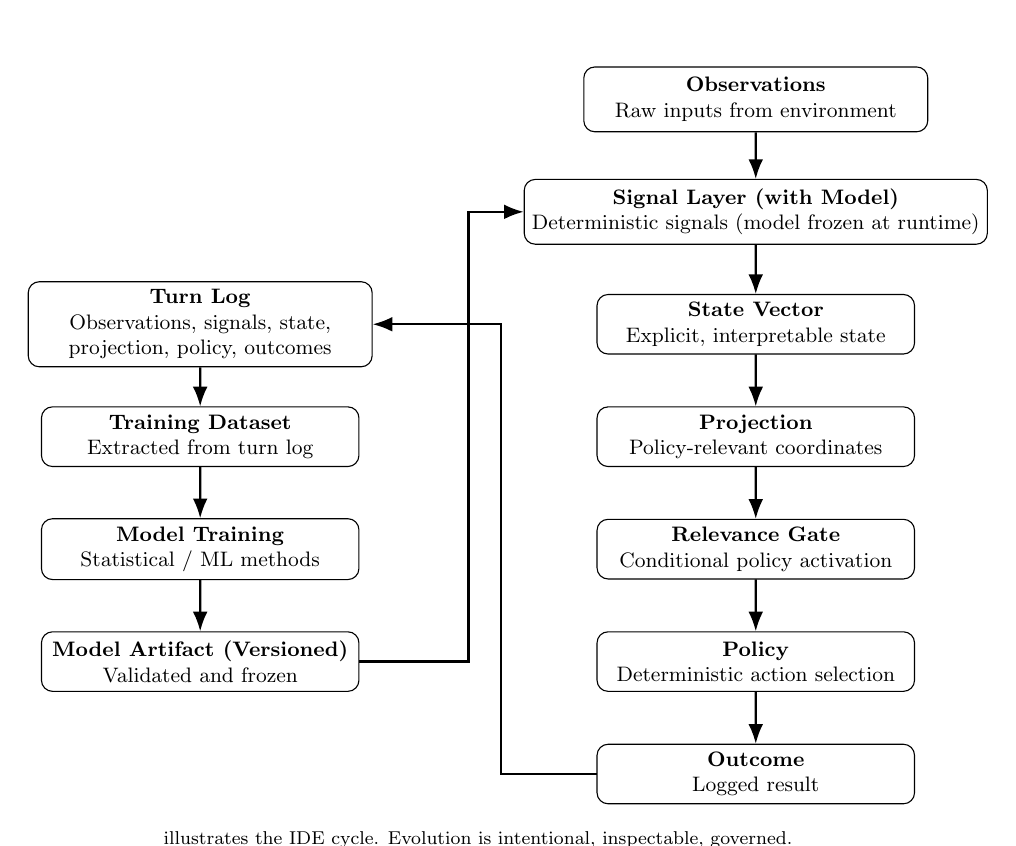
\begin{tikzpicture}[
  scale=0.84,
  transform shape,
  x=1cm, y=1cm,
  box/.style={
    rectangle,
    rounded corners,
    draw,
    align=center,
    minimum width=5.2cm,
    minimum height=0.98cm,
    font=\small
  },
  smallbox/.style={
    rectangle,
    rounded corners,
    draw,
    align=center,
    minimum width=4.8cm,
    minimum height=0.90cm,
    font=\small
  },
  note/.style={
    align=center,
    font=\footnotesize
  },
  arrow/.style={
    -{Latex[length=2.5mm]},
    thick
  }
]

% =========================================================
% Right column: runtime execution
% =========================================================
\node[box] (obs)    at (9.2, 8.6) {\textbf{Observations}\\Raw inputs from environment};

\node[box] (signal) at (9.2, 6.9) {\textbf{Signal Layer (with Model)}\\Deterministic signals (model frozen at runtime)};

\node[smallbox] (state)  at (9.2, 5.2) {\textbf{State Vector}\\Explicit, interpretable state};

\node[smallbox] (proj)   at (9.2, 3.5) {\textbf{Projection}\\Policy-relevant coordinates};

\node[smallbox] (gate)   at (9.2, 1.8) {\textbf{Relevance Gate}\\Conditional policy activation};

\node[smallbox] (policy) at (9.2, 0.1) {\textbf{Policy}\\Deterministic action selection};

\node[smallbox] (outcome) at (9.2, -1.6) {\textbf{Outcome}\\Logged result};

\draw[arrow] (obs) -- (signal);
\draw[arrow] (signal) -- (state);
\draw[arrow] (state) -- (proj);
\draw[arrow] (proj) -- (gate);
\draw[arrow] (gate) -- (policy);
\draw[arrow] (policy) -- (outcome);

% =========================================================
% Left column: offline training / refinement
% =========================================================
\node[box] (log) at (0.8, 5.2) {\textbf{Turn Log}\\Observations, signals, state, \\ projection, policy, outcomes};

\node[smallbox] (dataset) at (0.8, 3.5) {\textbf{Training Dataset}\\Extracted from turn log};

\node[smallbox] (train) at (0.8, 1.8) {\textbf{Model Training}\\Statistical / ML methods};

\node[smallbox] (model) at (0.8, 0.1) {\textbf{Model Artifact (Versioned)}\\Validated and frozen};

\draw[arrow] (log) -- (dataset);
\draw[arrow] (dataset) -- (train);
\draw[arrow] (train) -- (model);

% =========================================================
% Cross-column connections
% =========================================================

% Runtime outcomes recorded into turn log
\draw[arrow] (outcome.west) -- ++(-1.45,0) |- (log.east);

% Versioned model redeployed into signal/projection side
\draw[arrow] (model.east) -- ++(1.65,0) |- (signal.west);

% =========================================================
% Explanatory note
% =========================================================
\node[note] at (5.0, -2.6)
{illustrates the IDE cycle. Evolution is intentional, inspectable, governed.};

\end{tikzpicture}

\caption{Illustration of IDE cycle. Offline learning and runtime execution remain structurally separated. Evolution is intentional, inspectable, governed.}
\label{fig:esm-learning-loop}
\end{figure}

AI proposes refinements; humans authorize deployment. Policy authority $\pi$ remains deterministic---learning enriches interpretation, never bypasses decision boundary.

% ----------------------------
% Cybernetics Foundations
% ----------------------------
\section{Cybernetics Foundations}

ESM formalizes cybernetic principles within explicit, governable architecture:

\textbf{Cybernetics} established feedback regulation \cite{wiener1948, ashby1956}. ESM extends this by making \emph{signal construction} explicit---cybernetic "distinctions that make a difference" become versioned artifacts.

\textbf{Second-order cybernetics} emphasized observer-defined boundaries \cite{vonfoerster1974}. ESM operationalizes this: humans define signals $S_t$, projections $P$, desirable regions $\mathcal{Y}_D$, policies $\pi$.

\textbf{Complexity science} shows behavior emerges from local interactions \cite{wolfram2002}. ESM trajectories $\{T_1, T_2, \dots\}$ through committed states realize this via discrete turns, not continuous dynamics.

Key ESM extension: representational structure (signals $\to$ state $\to$ projection) becomes inspectable, versioned, governable. Traditional cybernetics treats perception as given; ESM makes it first-class architecture.

Policy $\pi(y_t)$ retains cybernetic feedback while governance spans full chain $o_t \to S_t \to x_t \to y_t \to g_t \to r_t$. System evolution becomes refinement of both behavior \emph{and} perception.

% ----------------------------
% Architecture Boundaries
% ----------------------------

\section{Architecture Boundaries}

ESM enforces structural separation but doesn't solve core modeling challenges. It's a decision \emph{architecture}, not a universal reasoning method.

\subsection{No Global Optimization}
Unlike dynamic programming over trajectories \cite{bellman1957}, ESM makes \emph{local} decisions: $\pi(y_t)$ evaluates present conditions only. Behavior emerges from turn sequences, not horizon optimization.

\subsection{Projection Depends on Signals}
Flawed signals $\to$ flawed $x_t$ $\to$ flawed $y_t$. Deterministic policy faithfully executes poor representations. ESM guarantees \emph{inspectability}, not correctness.

\subsection{Policy Design Remains Human}
$\pi(y_t)$ encodes normative judgment. Bad thresholds/escalation remain bad, but visible/revisable.

\subsection{Partial Observability}
No embedded POMDPs/belief states. Ambiguity $\to$ explicit clarification request (policy-triggered) or proceed under defined uncertainty. No probabilistic authority bypass.

\subsection{Generative AI Role}
LLMs assist signals/projection only $\to$ fixed explicit inputs. Never commit state/authorize $r_t$. Interpretation $\neq$ authority.

\subsection{Deployment Constraints}
Safety-critical: restrict $A$ to pre-authorized actions. Humans/supervisors retain final authority. ESM makes \emph{all} outcomes explicit/versioned.

ESM complements learning/optimization as \emph{governance framework} for consequential decisions requiring auditability/accountability.


% ----------------------------
% Related Work
% ----------------------------

\section{Related Work}
\label{sec:related_work}

ESM synthesizes control theory, cybernetics, and AI governance into explicit turn-based architecture.

\textbf{Control Theory}: Adopts state-space trajectories \cite{astrom2010} but replaces latent estimation with explicit signal $\to$ state $\to$ projection chain. Local policy $\pi(y_t)$ vs global optimization.

\textbf{System ID/Signal Processing}: Explicit signals $S_t$ replace learned features \cite{ljung1999}. Representation becomes governed construction, not inference.

\textbf{Representation Learning}: Committed state $x_t$ + projection $y_t = P(x_t)$ vs latent embeddings. Semantic transparency over efficiency.

\textbf{Decision Theory}: Externalizes uncertainty into explicit $x_t,y_t$ coordinates vs POMDP beliefs. Deterministic $\pi(y_t)$ under defined ambiguity.

\textbf{Naturalistic Decision Making}: Turn structure mirrors pattern recognition $\to$ policy response \cite{klein1998}.

\textbf{Event-Triggered Control}: Gating $g_t = G(y_t)$ generalizes conditional activation \cite{tabuada2007}.

\textbf{Hierarchical Systems}: Layered ESMs via explicit state handoff $x_1^{(d)} = H(x_{\text{handoff}}^{(u)}, o_1^{(d)})$ \cite{simon1962}.

\textbf{Distinguishing ESM Synthesis}:
\begin{itemize}
    \item \textbf{Coherent committed state} $x_t$ from explicit signals $S_t$
    \item \textbf{Projection} $y_t = P(x_t)$: no new semantics
    \item \textbf{Gating} $g_t$: explicit decision boundary  
    \item \textbf{Policy authority}: $\pi(y_t)$ sole $r_t$ producer
    \item \textbf{Structured deployment}: \emph{safe onboarding pathway} addressing knowledge acquisition bottlenecks via phased calibration and preference elicitation \cite{hoffman1987}
    \item \textbf{IDE}: versioned evolution via replay $\{T_i^{(v)} \leftrightarrow T_i^{(v')}\}$
\end{itemize}

ESM: governance architecture for consequential decisions, complementing (not replacing) learning/optimization.

% ----------------------------
% Conclusion
% ----------------------------
\section{Conclusion}

The Emergent State Machine (ESM) defines a deterministic architecture for interpretable situational reasoning through discrete \emph{turns}: $o_t \to S_t \to x_t \to y_t \to g_t \to r_t$.

Key contributions:
\begin{itemize}
\item \textbf{Coherent committed state} $x_t$: interpretation completes before decision
\item \textbf{Projection} $y_t = P(x_t)$: re-expresses without new semantics  
\item \textbf{Gating} $g_t = G(y_t)$: explicit decision boundary
\item \textbf{Policy authority}: $\pi(y_t)$ sole $r_t$ producer (no-op, action, escalation)
\item \textbf{Structured deployment}: \emph{safe onboarding pathway} for existing environments via phased calibration
\item \textbf{Instrumented Deterministic Evolution (IDE)}: versioned artifact revision via replay
\item \textbf{Layered ESMs}: explicit state handoff preserves modularity/traceability
\end{itemize}

Trajectories $\{T_1, T_2, \dots\}$ through policy space emerge from local decisions, analyzable via desirable regions $\mathcal{Y}_D$ without global optimization.

ESM doesn't solve modeling challenges but makes them \emph{explicit}: signals, projections, policies remain human-defined, inspectable, revisable. Probabilistic components inform interpretation; policy governs authority.

Reasoning becomes the object of governance. Turns enable analysis, replay, systematic evolution---transparent, accountable systems for consequential domains.

\bibliographystyle{plain}
\bibliography{references}
\end{document}
